\begin{block}{Atom-laser interaction}
  \begin{itemize}
  \item Cesium atom excited by a mode-locked laser
    \begin{itemize}
    \item Spectrum is a series of lines separated by the repetition rate: $f_n = n \Delta + \delta$
    \item Wide bandwith, can cover a large number of energy levels
    \end{itemize}
  \item Excited state linewidths are of the order of 700 MHz due to Doppler-broadening
  \end{itemize}
  \begin{columns}
    \begin{column}{0.49\textwidth}
      \begin{figure}
        \begin{center}
          \setlength\fboxsep{0pt}
          \setlength\fboxrule{0.5pt}
          \fbox{\includegraphics[width=.85\textwidth]{figures/energylevels}}
        \end{center}
      \end{figure}
      \begin{itemize}
      \item Coherent population trapping in the hyperfine ground states
      \item Excited state is on the D2 transition
      \item Input light is band-pass filtered with spatial light modulator (SLM) to reduce background scatter
      \end{itemize}
    \end{column}
    \begin{column}{0.49\textwidth}
      \begin{itemize}
      \item Simplified picture for CPT with mode-locked laser:
      \begin{figure}
        \begin{center}
          \setlength\fboxsep{0pt}
          \setlength\fboxrule{0.5pt}
          \fbox{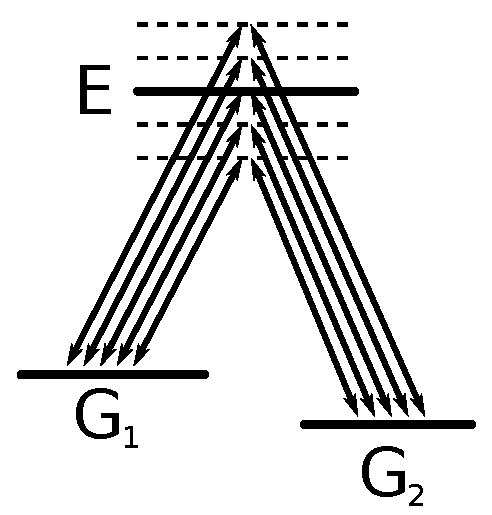
\includegraphics[width=.6\textwidth]{figures/modelockresonance}}
        \end{center}
      \end{figure}
      \begin{itemize}
       \item The mode-locked laser have multiple resonance conditions between the excited state E and the two ground states G$_1$ and G$_2$.
      \item Interaction is tuned by the repetition rate $\Delta$
      \end{itemize}
      \end{itemize}
    \end{column}
  \end{columns}
\end{block}
